\documentclass[aps,prb,twocolumn,superscriptaddress,amsmath,amssymb,floatfix]{revtex4}
%\documentclass[aps,prb,onecolumn,preprint,superscriptaddress,amsmath,amssymb,floatfix]{revtex4}
%\documentclass[aps,prl,onecolumn,groupedaddress,amsmath,amssymb,12pt]{revtex4}
\usepackage{graphicx}
\usepackage{ifthen}
\usepackage{dcolumn}% Align table columns on decimal point
\usepackage{bm}% bold math
\usepackage{multirow}
\usepackage{booktabs}
\usepackage{amsbsy}
\usepackage{amsmath}
\usepackage{amssymb}
\usepackage{subfigure}


%Definition of new commands
\newcommand{\f}[2]{\ensuremath{\frac{\displaystyle{#1}}{\displaystyle{#2}}}}
\newcommand{\lr}[1]{\langle{#1}\rangle}
\newcommand{\colv}[2] {\left(\begin{array}{c} #1 \\ #2 \end{array}\right)}
\renewcommand{\thefootnote}{\fnsymbol{footnote}}
\newcommand{\be} {\begin{eqnarray}}
\newcommand{\ee} {\end{eqnarray}}
%--------------------------------------------------------------------------
%EQ COMMANDS
%--------------------------------------------------------------------------
\newcommand{\two}{\mspace{-2.0mu}}
\newcommand{\four}{\mspace{-4.0mu}}
\newcommand{\plus}{\mspace{-4.5mu}+\mspace{-3.5mu}}
\newcommand{\minus}{\mspace{-4.5mu}-\mspace{-3.5mu}}
\newcommand{\pp}{'\mspace{-2.0mu}'}
\newcommand{\xlb}[4]{#1\ifthenelse{\equal{#2}{0}}{}{_{\alpha #2}}
\mspace{-2.0mu}\genfrac{(}{)}{0pt}{1}{\ifthenelse{\equal{#3}{0}}{0}{l #3}} 
{\ifthenelse{\equal{#4}{0}}{0}{b #4}}}

\newcommand{\xkv}[4]{#1\mspace{-5.0mu}\left(\mspace{-8.0mu}
\begin{smallmatrix}#2\four{}\four{}\mspace{-8.0mu}&\pmb{\kappa}#3\\&\nu 
#4\end{smallmatrix}\mspace{-5.0mu}\right)}

\newcommand{\evect}[6]{#1\mspace{-4.0mu}\left(\mspace{-8.0mu}
\begin{smallmatrix}#2\mspace{-8.0mu}&\pmb{\kappa} #3 &b #5\\&\nu #4 &
\alpha #6\end{smallmatrix}\mspace{-5.0mu}\right)}

\newcommand{\varmat}[8]{\mspace{-5.0mu}\left(\mspace{-8.0mu}
\begin{smallmatrix}\ifthenelse{\equal{#3}{0}}{\mspace{-8.0mu}&b_{#1}&b_{#2}
\\&\alpha_{#1}&\alpha_{#2}} {\ifthenelse{\equal{#7}{0}}{#1\mspace{-8.0mu}&
\pmb{\kappa}#2#3\mspace{-8.0mu}&\pmb{\kappa}#4#5\mspace{-8.0mu}&\pmb{\kappa}
#6\\&\nu#2&\nu#4&\nu#6} {#1\mspace{-8.0mu}&\pmb{\kappa}#2#3\mspace{-8.0mu}&
\pmb{\kappa}#4#5\mspace{-8.0mu}&\pmb{\kappa}#6#7\mspace{-8.0mu}&\pmb{\kappa}
#8\\&\nu#2&\nu#4&\nu#6&\nu#8}}\end{smallmatrix}\mspace{-5.0mu}\right)}

\newcommand{\EXP}[1]{\exp\mspace{-5.0mu}\left[#1\right]\mspace{-3.0mu}}

\newcommand{\tpp}[2]{\left(\mspace{-2.0mu}\xkv{\omega}{}{}{}#1\xkv{\omega}
{}{'}{'}#2\xkv{\omega}{}{\pp}{\pp}\mspace{-2.0mu}\right)}



%--------------------------------------------------------------------------
\newcommand{\SUM}[2]{\ifthenelse{\equal{#1}{0}}{\sum_{
\alpha_{#2},b_{#2},l_{#2}}^{3,n,N}} {\ifthenelse{\equal{#1}{1}}{\sum_{
\alpha_{#2},b_{#2}}^{3,n}}{\sum_{\pmb{\kappa}#2,\nu#2}^{N,3n}}}}

\newcommand{\SUMprime}[2]{\ifthenelse{\equal{#1}{0}}
{\sum_{\alpha_{#2},b_{#2},l_{#2}}^{3,n,N}} 
{\ifthenelse{\equal{#1}{1}}{\sum_{\alpha_{#2},b_{#2}}^{3,n}}
{\sum_{\pmb{\kappa}^{'}#2,\nu#2}^{N,3n}}}}

\newcommand{\SUMalpha}[2]{\ifthenelse{\equal{#1}{0}}
{\sum_{\alpha_{#2}}^{3}} {\ifthenelse{\equal{#1}{1}}
{\sum_{\alpha_{#2},b_{#2}}^{3,n}}{\sum_{\pmb{\kappa}#2,\nu#2}^{N,3n}}}}
%--------------------------------------------------------------------------
\newcommand{\SUMalphap}[2]{\ifthenelse{\equal{#1}{0}}
{\sum_{\alpha'_{#2}}^{3}} {\ifthenelse{\equal{#1}{1}}
{\sum_{\alpha'_{#2},b'_{#2}}^{3,n}}{\sum_{\pmb{\kappa}#2,\nu#2}^{N,3n}}}}

\newcommand{\SUMb}[2]{\ifthenelse{\equal{#1}{0}}{\sum_{b_{#2}}^{n}}
 {\ifthenelse{\equal{#1}{1}}{\sum_{\alpha_{#2},b_{#2}}^{3,n}}
{\sum_{\pmb{\kappa}#2,\nu#2}^{N,3n}}}}

\newcommand{\SUMbp}[2]{\ifthenelse{\equal{#1}{0}}{\sum_{b'_{#2}}^{n}}
 {\ifthenelse{\equal{#1}{1}}{\sum_{\alpha'_{#2},b'_{#2}}^{3,n}}
{\sum_{\pmb{\kappa}#2,\nu#2}^{N,3n}}}}

\newcommand{\SUMl}[2]{\ifthenelse{\equal{#1}{0}}{\sum_{l_{#2}}^{N}}
 {\ifthenelse{\equal{#1}{1}}{\sum_{\alpha_{#2},b_{#2}}^{3,n}}
{\sum_{\pmb{\kappa}#2,\nu#2}^{N,3n}}}}

\newcommand{\SUMlp}[2]{\ifthenelse{\equal{#1}{0}}{\sum_{l'_{#2}}^{N}}
 {\ifthenelse{\equal{#1}{1}}{\sum_{\alpha'_{#2},b'_{#2}}^{3,n}}
{\sum_{\pmb{\kappa}#2,\nu#2}^{N,3n}}}}

\newcommand{\abcdt}[5]{\mspace{-4.0mu}\left(\mspace{-8.0mu}
\begin{smallmatrix}&\ifthenelse{\equal{#1}{}}{a}{#1}&\ifthenelse
{\equal{#3}{}}{c}{#3}\\&\ifthenelse{\equal{#2}{}}{b}{#2}&\ifthenelse
{\equal{#4}{}}{d}{#4}\end{smallmatrix}\mspace{-2.0mu};\ifthenelse
{\equal{#5}{}}{t}{#5}\right)}

\newcommand{\abcd}[4]{\mspace{-4.0mu}\left(\mspace{-8.0mu}
\begin{smallmatrix}&\ifthenelse{\equal{#1}{}}{a}{#1}&\ifthenelse
{\equal{#3}{}}{c}{#3}\\&\ifthenelse{\equal{#2}{}}{b}{#2}&\ifthenelse
{\equal{#4}{}}{d}{#4}\end{smallmatrix}\mspace{-3.0mu}\right)}

\newcommand{\abt}[3]{\mspace{-4.0mu}\left(\mspace{-8.0mu}\begin
{smallmatrix}&\ifthenelse{\equal{#1}{}}{a}{#1} \\&\ifthenelse{
\equal{#2}{}}{b}{#2}\end{smallmatrix}\mspace{-2.0mu};
\ifthenelse{\equal{#3}{}}{t}{#3}\right)}

\newcommand{\ab}[2]{\mspace{-4.0mu}\left(\mspace{-8.0mu}
\begin{smallmatrix}&\ifthenelse{\equal{#1}{}}{a}{#1} \\&\ifthenelse
{\equal{#2}{}}{b}{#2}\end{smallmatrix}\mspace{-3.0mu}\right)}

\newcommand{\kvbat}{\mspace{-4.0mu}\left(\mspace{-8.0mu}
\begin{smallmatrix} &\pmb{\kappa} &b \\ &\nu &\alpha\end{smallmatrix}
\mspace{-2.0mu};t\right)}
%--------------------------------------------------------------------------
\newcommand{\kvbatp}{\mspace{-4.0mu}\left(\mspace{-8.0mu}
\begin{smallmatrix} &\pmb{\kappa} &b' \\ &\nu &\alpha'\end{smallmatrix}
\mspace{-2.0mu};t\right)}

\newcommand{\kvbaw}{\mspace{-4.0mu}\left(\mspace{-8.0mu}
\begin{smallmatrix} &\pmb{\kappa} &b \\ &\nu &\alpha\end{smallmatrix}
\mspace{-2.0mu};\omega\right)}

\newcommand{\kvbawp}{\mspace{-4.0mu}\left(\mspace{-8.0mu}
\begin{smallmatrix} &\pmb{\kappa} &b' \\ &\nu &\alpha'\end{smallmatrix}
\mspace{-2.0mu};\omega\right)}

\newcommand{\kvba}{\mspace{-4.0mu}\left(\mspace{-8.0mu}
\begin{smallmatrix} &\pmb{\kappa} &b \\ &\nu &\alpha\end{smallmatrix}
\mspace{-3.0mu}\right)}

\newcommand{\kvbap}{\mspace{-4.0mu}\left(\mspace{-8.0mu}
\begin{smallmatrix} &\pmb{\kappa}' &b \\ &\nu' &\alpha\end{smallmatrix}
\mspace{-3.0mu}\right)}
%--------------------------------------------------------------------------
\newcommand{\kpvba}{\mspace{-4.0mu}\left(\mspace{-8.0mu}
\begin{smallmatrix} &\pmb{\kappa}^{'} &b \\ &\nu &\alpha\end{smallmatrix}
\mspace{-3.0mu}\right)}

\newcommand{\kva}{\mspace{-4.0mu}\left(\mspace{-8.0mu}
\begin{smallmatrix} &\pmb{\kappa} \\ &\nu &\alpha\end{smallmatrix}
\mspace{-3.0mu}\right)}

\newcommand{\kvap}{\mspace{-4.0mu}\left(\mspace{-8.0mu}
\begin{smallmatrix} &\pmb{\kappa} \\ &\nu &\alpha'\end{smallmatrix}
\mspace{-3.0mu}\right)}

\newcommand{\kvb}{\mspace{-4.0mu}\left(\mspace{-8.0mu}
\begin{smallmatrix} &\pmb{\kappa} &b \\ &\nu \end{smallmatrix}
\mspace{-3.0mu}\right)}

\newcommand{\kvbp}{\mspace{-4.0mu}\left(\mspace{-8.0mu}
\begin{smallmatrix} &\pmb{\kappa} &b' \\ &\nu \end{smallmatrix}
\mspace{-3.0mu}\right)}

\newcommand{\kvt}{\mspace{-4.0mu}\left(\mspace{-8.0mu}
\begin{smallmatrix}&\pmb{\kappa} \\&\nu\end{smallmatrix}
\mspace{-2.0mu};t\right)}

\newcommand{\kvzero}{\mspace{-4.0mu}\left(\mspace{-8.0mu}
\begin{smallmatrix}&\pmb{\kappa} \\&\nu\end{smallmatrix}
\mspace{-2.0mu};0\right)}

\newcommand{\kpvt}{\mspace{-4.0mu}\left(\mspace{-8.0mu}
\begin{smallmatrix}&\pmb{\kappa}^{'} \\&\nu\end{smallmatrix}
\mspace{-2.0mu};t\right)}

\newcommand{\kvw}{\mspace{-4.0mu}\left(\mspace{-8.0mu}
\begin{smallmatrix}&\pmb{\kappa} \\&\nu\end{smallmatrix}
\mspace{-2.0mu};\omega\right)}

\newcommand{\kv}{\mspace{-4.0mu}\left(\mspace{-8.0mu}
\begin{smallmatrix}&\pmb{\kappa} \\&\nu\end{smallmatrix}
\mspace{-3.0mu}\right)}

\newcommand{\kvp}{\mspace{-4.0mu}\left(\mspace{-8.0mu}
\begin{smallmatrix}&\pmb{\kappa'} \\&\nu'\end{smallmatrix}
\mspace{-3.0mu}\right)}

\newcommand{\kw}{\mspace{-4.0mu}\left(\mspace{-8.0mu}
\begin{smallmatrix}&\pmb{\kappa} \\&\omega\end{smallmatrix}
\mspace{-3.0mu}\right)}

\newcommand{\kpvp}{\mspace{-4.0mu}\left(\mspace{-8.0mu}
\begin{smallmatrix}&\pmb{\kappa'} \\&\nu'\end{smallmatrix}
\mspace{-3.0mu}\right)}
%--------------------------------------------------------------------------
\newcommand{\lbt}{\mspace{-4.0mu}\left(\mspace{-8.0mu}
\begin{smallmatrix}&l \\&b\end{smallmatrix}\mspace{-2.0mu};t\right)}

\newcommand{\lbtp}{\mspace{-4.0mu}\left(\mspace{-8.0mu}
\begin{smallmatrix}&l' \\&b'\end{smallmatrix}\mspace{-2.0mu};t\right)}

\newcommand{\lt}{\mspace{-4.0mu}\left(\mspace{-8.0mu}
\begin{smallmatrix}&l\end{smallmatrix}\mspace{-2.0mu};t\right)}

\newcommand{\ltp}{\mspace{-4.0mu}\left(\mspace{-8.0mu}
\begin{smallmatrix}&l'\end{smallmatrix}\mspace{-2.0mu};t\right)}

\newcommand{\lb}{\mspace{-4.0mu}\left(\mspace{-8.0mu}
\begin{smallmatrix}&l \\&b\end{smallmatrix}\mspace{-3.0mu}\right)}

\newcommand{\lbp}{\mspace{-4.0mu}\left(\mspace{-8.0mu}
\begin{smallmatrix}&l' \\&b'\end{smallmatrix}\mspace{-3.0mu}\right)}
%--------------------------------------------------------------------------
%COMMANDS
%--------------------------------------------------------------------------

%--------------------------------------------------------------------------
\begin{document}
%--------------------------------------------------------------------------

%--------------------------------------------------------------------------
\title{Evaluation of the Virtual Crystal Approximation for Predicting 
Thermal Conductivity}
%--------------------------------------------------------------------------
\author{Jason M. Larkin}
\affiliation{Department of Mechanical Engineering\\Carnegie Mellon 
University\\Pittsburgh, PA 15213}
\author{A. J. H. McGaughey}
\email{mcgaughey@cmu.edu}
\affiliation{Department of Mechanical Engineering\\
Carnegie Mellon University\\Pittsburgh, PA 15213}
%--------------------------------------------------------------------------

%--------------------------------------------------------------------------
\date{\today}
%--------------------------------------------------------------------------


%--------------------------------------------------------------------------
\begin{abstract}
%--------------------------------------------------------------------------
In this work, the virtual crystal approximation for mass disorder is 
evaluated by examining two model alloy systems: Lennard-Jones argon 
and Stillinger-Weber silicon. In both cases the perfect crystal is 
alloyed with a heavier mass species up to equal concentration and 
phonon properties and thermal conductivity 
are precited. These 
two alloyed systems have different ranges of phonon frequencies, 
lifetimes, and mean free paths.
For Stillinger-Weber silicon, the 
virtual crystal approximation predicts phonon properties and thermal 
conductivity in good agreement with molecular dynamics-based methods. 
For Lennard-Jones argon, the virtual crystal approximation underpredicts 
the high frequency phonon lifetimes, leading to an underpredicting of 
its thermal conductivity. Resolution of these underpredictions is achieved 
by consindering methods which treat the disorder explicitly. 
%--------------------------------------------------------------------------
\end{abstract}
%--------------------------------------------------------------------------


%--------------------------------------------------------------------------
\maketitle
%--------------------------------------------------------------------------
\clearpage
%--------------------------------------------------------------------------
\section{\label{S:Introduction}Introduction}
%--------------------------------------------------------------------------

Accurately predicting the thermal conductivity of a dielectric or 
semiconducting material requires the properties of phonons from the entire 
Brillouin zone. Accurate predictions of phonon properties for bulk systems 
can be made with anharmonic lattice dynamics theory using ab initio 
calculations.\cite{
broido_intrinsic_2007,ward_ab_2009,ward_intrinsic_2010,lindsay_thermal_2012,
garg_role_2011,
shiga_microscopic_2012,tian_phonon_2012,shiomi_thermal_2011}
However, computational costs limit the size of computational cells 
in ab initio calculations to be less than 100 atoms, making it difficult 
to directly incorporate the effects of disorder.
\cite{koker_thermal_2009,bao_first-principles_2012,
lindsay_thermal_2012,tian_phonon_2012,garg_role_2011}
Alternatively, theory 
that treats disorder as a harmonic perturbation can be used to estimate 
the reduction in phonon lifetimes due to disorder scattering without 
the use of a large unit cell.
\cite{tian_phonon_2012,garg_role_2011,lindsay_thermal_2012}
Under this approximation, the disordered 
crystal is replaced with a perfect “virtual crystal” with properties 
equivalent to an averaging over the disorder (e.g.  mass or bond 
strength).\cite{abeles_lattice_1963}

Recently, work using ab-initio calculations, anharmonic 
lattice dynamics (ALD) and the virtual crystal (VC) 
approximation was used to predict phonon mode frequencies, lifetimes and 
group velocities of materials with realtively
large,\cite{garg_role_2011,lindsay_thermal_2012} 
moderate,\cite{thermal_shiomi_2011}, and 
small \cite{tian_phonon_2012} 
thermal conductivities. The use of ALD and VC (referred to as VC-ALD) 
treats the effects of intrinsic and disorder scattering as perturbations 
rather than including disorder explicitly.(cite)
However, no comprehensive study has been performed 
to assess the applicability of this perturbative approach for a range 
of heavily disorered systems using multiple predictive methods.

In intro, mention taud model, VC vs. Gamma point, NMD technique.

The goal of this work is to verify the use of the VC 
approximation for predicting thermal conductivity by a detailed comparison 
of 3 predictive methods: MD-based normal mode 
decomposition (NMD) and green-kubo (GK), 
and VC-ALD which treats the harmonic and 
anharmonic phonon scattering as perturbations 
(Section \ref{S:From VC-ALD}). 
When used with the VC 
approximation, methods are referred to as VC-NMD and VC-ALD.
Two model binary-alloy systems 
with varying concentrations ($c$) of mass defects ($m^a_{1-c}m^b_{c}$) 
are considered: 
Lennard-Jones (LJ) argon and Stillinger-Weber (SW) silicon. 
In both cases the perfect crystal is 
alloyed with a heavier mass species up to equal concentration, spanning 
a range of perturbative to heavy disorder. These 
two alloyed systems have very different ranges of phonon frequencies, 
lifetimes, group velocities and total thermal conuctivity. 
For SW silicon, 
VC-ALD predicts thermal conductivity in good agreement with GK. 
For LJ argon, the VC-ALD approximation underpredicts 
the high frequency phonon lifetimes, leading to an underpredicting of 
the thermal conductivity. The different thermal conductivity spectra of 
and the breakdown of the perturbative models are examined.

%--------------------------------------------------------------------------
\section{\label{S:Virtual Crystal}Virtual Crystal (VC) Approximation}
%--------------------------------------------------------------------------

%--------------------------------------------------------------------------
\subsection{\label{S:Overview}Overview}
%--------------------------------------------------------------------------

Abeles first introduced the idea of using a virtual crystal (VC) to 
replace a disordered one, computing the
thermal conductivity of Si/Ge alloys by treating both
disorder and anharmonicity as perturbations.\cite{abeles_lattice_1963} 
Many experimental trends in thermal conductivity 
of a range of materials 
can be explained using the VC approximation.(cite) For example,
the reduced thermal conductivity of Ge versus Si and Si/Ge alloys 
is partly explained 
by both the increased mass and decreased bulk modulus (stiffness) of the 
lattice.(cite) Both have the effect of reducing phonon group velocities.
(cite) However, a complete 
description of the thermal transpot in alloys requires modeling intrinsic 
and disordered scattering to calculate phonon lifetimes 
(see Section \ref{S:From VC-ALD}).

Phonon lifetimes can be predicted by treating both the intrinsic 
and disorder scattering using perturbation theory (Section ). 
While the theory which treats phonon defect scattering (Eq. ) 
is valid for
perturbative disorder, its use leads to good agreement with
several experimental and computational results with large disorder.  
Cahill shows that conductivty reduction in dilute 
Ge-doped Si epitaxial layers 
is captured by mass perturbative disorder.
\cite{cahill_thermal_2004cahill_thermal_2005} 
While the mass disorder was large ($m_{Ge}/m_{Si} = 2.6$),  
the overall disorder strength is dictated by the concentration. 
As little as $6.2\times10^{19} cm^{-3}$ Ge
($g = 3.1\times10^{-3}$, Section ) 
is enough to reduce the thermal conductivity of 
Si by almost a factor of 2.\cite{cahill_thermal_2004}
In the
case of the $Ni_{0.55}Pd_{0.45}$ alloy, the atomic species
are chemically similar but both the mass disorder 
($m_{Pd}/m_{Ni} \approx 2$) and concentration are large ($g=0.078$) 
and good agreement is also seen using a VC approach.
\cite{kamitakahara_vibrations_1974}

Computational results using the VC approximation 
for moderate to high thermal conductivity 
alloys show good to excellent agreement with experimental results
\cite{thermal_shiomi_2011,garg_role_2011,lindsay_thermal_2012}.
Garg used ab initio calculations with VC-ALD (Section )  
to predict the thermal conductivity of Si/Ge alloys 
for all concentrations, obtaining excellent agreement with experiment.
\cite{garg_role_2011}  Lindsay and Broido 
found good agreement with VC-ALD and experiment for 
isotopically defected GaN.\cite{lindsay_thermal_2012}  
Both Si/Ge and isotopically defected GaN have relatively large 
thermal conductivities, even for large concentrations.
A detailed study of low thermal conductivity materials 
PbTe\cite{shiga_microscopic_2012} and PbTe/PbSe\cite{tian_phonon_2012} 
made predictions for the perfect systems in fair agreement with experiment, 
but where results lack for the alloys. 
Thus, there is a need to 
examine the perturbative approach VC-ALD for heavily disordered 
systems. 
The computational studies discussed above were limited to the use 
of VC-ALD because of the computational cost of ab initio calcualtions. 
Using empirical potentials, we study the effects of explicit 
disorder in Section .

Using the VC approximation, 
we perform calculations at different concentations ($c$) 
of mass varying ($m^a_{1-c}m^b_{c}$) binary alloys of LJ argon 
and SW silicon (Section ). Using the VC approximation, 
the phonon mode properties of the VC 
(frequencies (Section ) and group velocities (Section )) 
and predict lifetimes (Section ) and thermal
conductivity (Section ). Methods referred to as VC-NMD (Section )
and VC-ALD (Section ) use the VC approximation. Explicit disorder 
is examined using lattice dynamics (LD) calculations 
(Section ) and molecular dynamics (MD) simulations 
(Section ) of explicitly disordered supercells (Section ). 

%--------------------------------------------------------------------------
\begin{figure}
\begin{center}
\mbox{\subfigure{(a)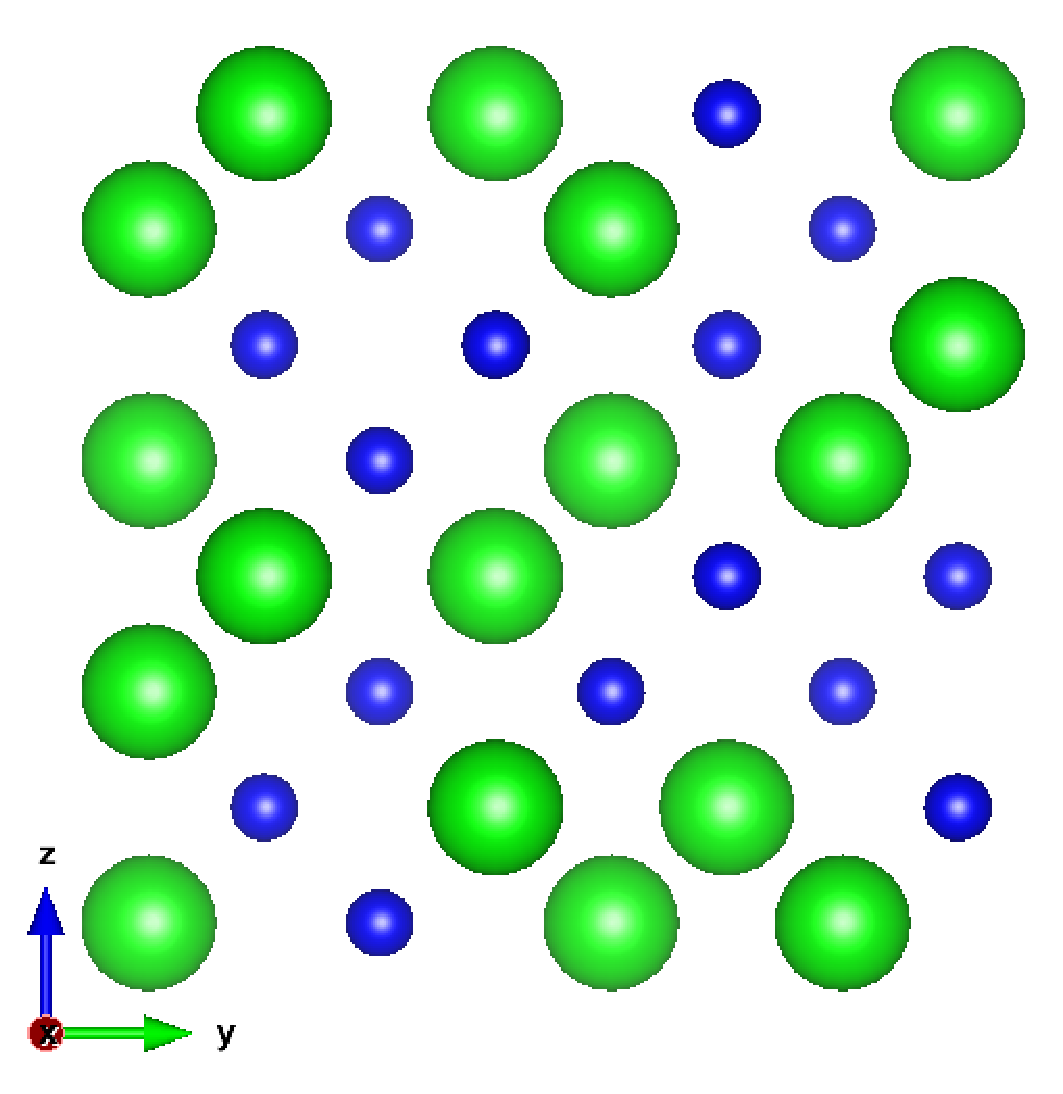
\includegraphics[scale=0.2]
{/home/jason/disorder/si/si_conv_2x2x2_disorder-2.eps}
\subfigure{(b)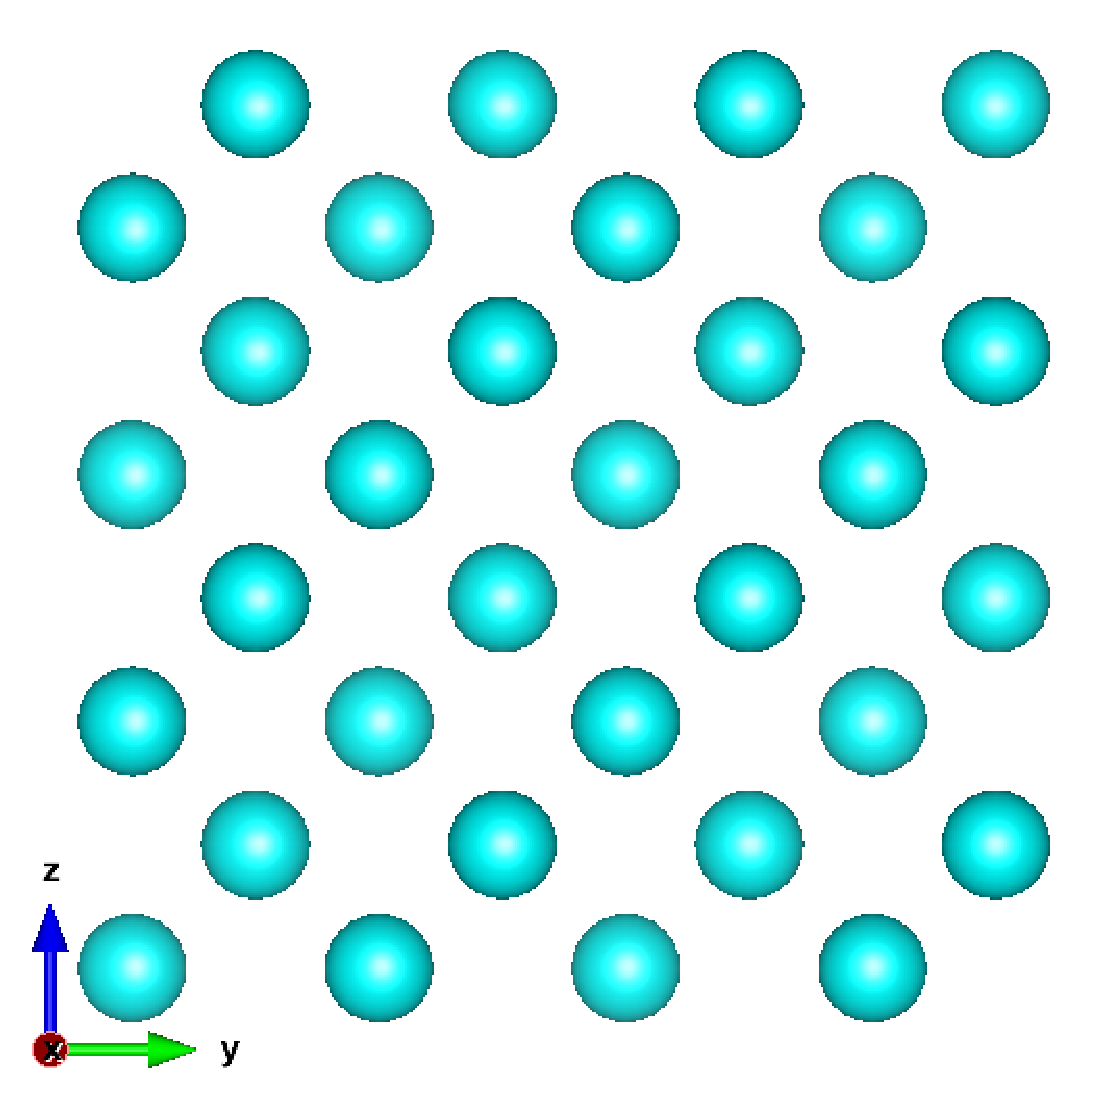
\includegraphics[scale=0.2]
{/home/jason/disorder/si/si_conv_2x2x2_perfect-2.eps}}}}
\vspace*{0mm}
\end{center}
\caption{\label{F:supercells} 
(a) view of a [010][001] plane of  
an explicitly disoredered supercell of 
Si and ``heavy'' Si ([100] direction into the paper).
\cite{momma_vesta:_2008} 
(b) view of a [010][001] plane of the VC supercell 
with an average
mass of the explicitly disordered Si and ``heavy'' Si supercell 
(b). 
Sphere size represents 
increasing mass 
only, no bond disorder is considered. 
In this work, calculations for LJ Ar and SW Si which use the VC 
approximation 
are based off of the conventional cubic unit cells 
(Section \ref{S:VC Gamma DOS}, \ref{S:From VC Dispersion}, 
\ref{S:From VC Gamma} and \ref{S:From VC-ALD}), 
which build the lattice of the perfect (a) 
and disordered supercells (b). 
Disorder is taken into account explicitly using the disordered 
supercells in Sections 
\ref{S:VC Gamma DOS}, \ref{S:From Structure Factor},  
\ref{S:From VC Gamma} and \ref{S:Diffuson Mode Diffusivity}. 
}
\end{figure}

%--------------------------------------------------------------------------


%--------------------------------------------------------------------------
\subsection{\label{S:Kinetic Theory}Kinetic Theory}
%--------------------------------------------------------------------------

For a perfect system, all vibrational modes are phonons, which by 
defintion are delocalized, propagating plane waves.(cite)  
Using the single-mode relaxation
time approximation \cite{ziman_electrons_2001} as an approximate solution of
the Boltzmann transport equation \cite{peierls_quantum_2001} gives an 
expression for thermal conductivity,
\begin{equation}\label{EQ:k_vib}
\begin{split}
k_{ph,\mathbf{n}}=&\sum_{\pmb{\kappa}} \sum_\nu c_{ph}\kv 
\pmb{v}^{2}_{g,\mathbf{n}}\kv \tau\kv.
\end{split}
\end{equation}
Here, the phonon mode has frequency $\omega\kv$ (Section ), 
$c_{ph}$ is the phonon volumetric specific heat, 
${v}_{g,\mathbf{n}}$ is
the component of the group velocity vector in direction $\mathbf{n}$ 
(Section ), 
and $\tau\kv$ is the phonon lifetime (Section ).
Since the MD simiulations we perform (Section ) are classical 
and obey Maxwell-Boltzmann 
statistics,\cite{mcquarrie_statistical_2000} the
specific heat is $k_{B}/V$ per mode in the harmonic limit, where $V$ 
is the system volume. This approximation has been shown to be valid 
for LJ Ar(cite SED or ASME?) and SW Si(cite SED or ASME?) 
and is used for all calculations 
in this work so that direct comparisons can be made for all methods.
(cite SED or AMSE?) For the perfect and disordered lattices studied 
in this work, the thermal conductivity is isotropic so we refer to 
$k_{ph}$ only.

For heavily disordered systems, the Allen-Feldman theory computes 
the contribution to vibrational 
conducitvity by diffuson modes (Section ).
\cite{allen_thermal_1993} 

Studies have attempted to quantify 
the relative contribution of both phonons and diffusons 
to the total vibrational 
conductivity, $k_{vib} = k_{ph} + k_{AF}$.\cite{he_heat_2011}

energy transport in jammed sphere packings\cite{xu_energy_2009}

heat transport in model jammed solids\cite{vitelli_heat_2010}

%--------------------------------------------------------------------------
\subsection{\label{S:VC Gamma DOS}VC and Gamma DOS}
%--------------------------------------------------------------------------

In this section, we examine the effect of explicit disorder by computing 
the density of states (DOS, $D(\omega\kv)$) for vibrational modes of  
the VC and of explicitly disordered supercells. 
Perfect and explicitly disordered supercells are generated 
with atomic positions 
based on LJ argon's FCC and silicon's diamond-FCC ($b\le8$) 
crystal structure using randomized masses.
The composition is labeled by $m^a_{1-c}m^b_{c}$,  
where $m^a=1$ and $m^b=3$ in 
LJ units for argon and $m^a=m_{Si}$ and $m^b=2.6m_{Si}$ 
for SW silicon and ``heavy silicon'' (mass of germanium). 
For $c=0.5$, the LJ VC has average mass of 2. 

Supercells are built cubically with size $N_0$, where $N_0$ refers to the 
number of repetitions of the unit cell in all 3 
spatial directions.(cite) Supercells up to size $N_0 \le 12$ 
for LJ argon (6096 atoms) are used for calculations. For SW silicon, 
$N_0 \le 10$ (SW silicon, 8000 atoms) are used for 
the MD-based methods and $N_0 \le 24$ for VC-ALD.  
The lattices are generated using the  
cubic conventional unit cells of the FCC ($n=4$) and 
diamond-FCC ($n=4$) crystals (where $n$ the number of atoms 
in the unit cell).

The supercells are built using 
the zero-pressure finite-temperature lattice constants 
for LJ argon, which are $a=1.556$ (T=10K) and 
and $a=1.580$ (T=40 K) in LJ units. 
For LJ argon, the variation of lattice constant 
with composition is small and ignored. 
The effective zero-pressure finite-temperature 
lattice constant 
of the amorphous phase at T=10K is slightly larger 
($a = 1.585 = (1/n_{v})^(1/3)$ where  
$n_{v}$ is the number density, Section ) and does not 
exist above approximately $T=20K$.\cite{mcgaughey} 
All LJ calculations use these lattice constants. 
For SW silicon, the lattice constant $a=5.43 \AA$ is used 
for all calculations, which brings the GK thermal conductivty 
predictions\cite{goicochea_thermal_2010} 
into better agreement with VC-ALD
\cite{sellan_cross-plane_2010}, particularly 
for $c=0.0$ (Section ).

Each vibrational mode contributing to the thermal conductivity 
has a frequency $\omega\kv$. The allowed frequencies 
are the sqaure root of the 
eigenvalues of the system's Dynamical matrix,
$D(\mathbf{\kappa})$,\cite{dove_introduction_1993}  
which relates the mode eigenvector ($e\kvba$) 
and eigenvalue by
\begin{equation}\label{EQ:Dynamical}
D(\mathbf{\kappa}) e\kvba = \omega^2\kv e\kvba.
\end{equation}
In a perfect system all vibrational (normal) modes are 
plane-waves, and as such 
can be identified by a wave-vector  
$\mathbf{\kappa}$, eigenvector $e\kvba$, and a possibly 
degenerate frequency $\omega\kv$. Here, $b$ labels the atom in the unit cell, 
$\alpha$ labels the cartesian coordiantes, and $\nu$ labels the mode 
polarization (possibly degenerate in frequency). 
In a disordered system, such as a 
crystal lattice with randomly arranged and differing mass species, 
all normal modes exist at the wavevector $[000]$, where $b \le N_{a}$ 
and $\nu \le 3N_a$, where $N_a$ is the total number of atoms in the system. 
In general, 
normal modes in a disordered system will not be pure plane-waves and 
will be non-degenerate in frequency. We compare the ordered and disordered 
normal mode frequencies in Section \ref{S:vc_gamma_dos} and 
mode eigenvectors in Section .

With the appropriate dynamical matrix 
($\mathbf{\kappa} = [000]$ for the 
explicitly disordered supercells), the frequencies 
are computed using the program GULP.\cite{gale_general_2003} For the 
VC, the frequencies are identified (up to polarization) by 
the list of wavevectors allowed by the size of the 
supercell.(cite) 
The DOS for the VC and the explicitly disordered supercells 
(referred to as Gamma) are shown in Fig. The frequencies agree between 
VC and Gamma at low frequencies, where the Debye approximation predicts 
$DOS(\omega) \propto \omega^2$.(cite) The increasing lattice 
mass with increasing $c$ for the VC has the effect of reducing 
the frequencies. The increasing lattice 
mass for the Gamma modes also has the effect of 
reducing the frequencies.
However, 
the effect of expicit disorder can be seen at high frequencies by a 
broadening and a shift of the DOS to higher frequencies 
because of the explicit light atoms used in the supercell. 
Similar agreement at low frequencies was found in ab initio predictions 
for $Si_cGe_{1-c}$,\cite{garg_role_2011} while Bouchard showed similar 
behavior for a-$Si_cGe_{1-c}$.\cite{bouchard_vibrational_1988} 

%--------------------------------------------------------------------------
\begin{figure}
\begin{center}
\includegraphics[scale=0.8]
{/home/jason/disorder/lj/alloy/lj_alloy_dos_c05-5_4.eps}
\vspace*{-5mm}
\end{center}
\caption{\label{F:DOS} Density of states (DOS) 
for modes calculated using the LJ FCC  
VC versus an explcitily mass disordered LJ FCC supercell 
(labeled Gamma) with varying mass concentration $c$ (Section ). 
VC and Gamma show similar low frequency behavior for all $c$. 
For increasing $c$, the frequencies of both VC 
and Gamma decrease, while the high frequency DOS for Gamma spreads and  
reaches up to a higher maximum frequency because of the explict disorder. 
The size of these supercells is $N_0 = 12$ (see Section ).
}
\end{figure}
%--------------------------------------------------------------------------

%--------------------------------------------------------------------------
\subsection{\label{S:Phonon Group Velocities}
Phonon Group Velocities}
%--------------------------------------------------------------------------

%--------------------------------------------------------------------------
\subsubsection{\label{S:From VC Dispersion}From VC Dispersion}
%--------------------------------------------------------------------------

The group velocity vector in a VC is the gradient of the dispersion curves 
(i.e., $\partial \omega / \partial \pmb{\kappa}$), which can be 
calculated from the frequencies and wavevectors using finite differences. 
In this work, the group velocities for the VC are calculated 
using finite difference 
and quasi-harmonic lattice dynamics.\cite{mcgaughey2006b} 
While the group 
velocities are necessary to predict the thermal conductivity, 
of particular interest is the phonon mean free path (MFP), 
$\Lambda\kv = |\pmb{v}_{g}| \tau\kv$, which is crucial for understanding 
nano and micro-nanostructuring effects.(cite) Thus, predicting 
group velocities in disordered systems is just as crucial as 
predicting mode lifetimes.(cite)

Except for the three 
acoustic branches (2 transverse, 1 logitudinal), there is not an 
accepted method to calculate the effective group velocity of a 
vibrational mode in a disordered system. though there are attempts.
\cite{duda_reducing_2011,donadio_atomistic_2009,
he_heat_2011,he_thermal_2011} 
Dispersion for a model 1D system demonstrated the effect of disorder 
on the group velocity in terms of a 
zone-folding effect.\cite{duda_reducing_2011} 
In studies of disordered silicon systems, the group velocity of 
vibational modes was estimated using an interpolation scheme for 
small but finite wavevectors 
around [000]. 
\cite{donadio_atomistic_2009,he_heat_2011,he_thermal_2011} 
We do not, in general, observe the required dispersion beavhior 
to perform this interpolation for the LJ and SW systems 
studied in this work. 
Feldman et al used the structure factor to predict an effective dispersion 
for a model of a-Si, but did not predict group velocities.(cite)  
Volz and Chen used the dynamical structure factor to predict the
dispersion of SW Si using MD simulation, but in a perfect system.
\cite{chen_molecular-dynamics_2000} We examine the structure factor for the 
explictily disordered modes in the next section.

%--------------------------------------------------------------------------
\subsubsection{\label{S:From Structure Factor}
From Structure Factor of Gamma Modes}
%--------------------------------------------------------------------------

Measuring the explicitly disordered (Gamma)  
mode's structure factor is a method to test for the plane-wave 
character of modes at a particular wavevector and polarization.(cite) 
The structure factor is defined as\cite{allen_diffusons_1999} 
\begin{equation}\label{EQ:SLT}
S^{L,T}\kw = 
\sum_{\nu} E^{L,T}\kv
\delta (\omega-\omega\kv),
\end{equation}
where $E^{T}$ refers to transverse polarization and is defined as
\begin{equation}\label{EQ:EL}
E^L\kv = 
\left|
\sum_{l,b} 
\hat{\mathbf{\kappa}} \cdot e\kvba 
\EXP{i\pmb{\kappa}\cdot\mathbf{r}_0\ab{l}{b}} 
\right|^2
\end{equation}
and $E^{L}$ refers to logitudinal polarization and is defined as
\begin{equation}\label{EQ:ET}
E^T\kv = 
\left|
\sum_{l,b} 
\hat{\mathbf{\kappa}} \times e\kvba 
\EXP{i\pmb{\kappa}\cdot\mathbf{r}_0\ab{l}{b}} 
\right|^2.
\end{equation}
Here, $\mathbf{r}_0\ab{l}{b}$ refers to the lattice positions in the 
mass disordered supercells which are still spaitally ordered. 
Explicit disorder is accounted for in the mode frequencies $\omega\kv$ 
and eigenvectors $e\kvba$ which are calculated with 
$\mathbf{\kappa} = [000]$. 

Physically, $S^{L,T}\kw$ calculates 
the frequency spectrum required to create a wavepacket with 
well-defined wavevector and polarization. In a perfect system the 
structrue factor peaks are delta functions centered at the mode 
frequencies. 
With increasing disorder ($c$), the structure factor spreads in width,  
particularly at high frequencies (Fig ). 
An effective dispersion can be extracted by locating the peaks in the 
structure factors, where the effects of polarization, virtual mass, and 
anisotropic dispersion can be observed (Fig. ). 
As the lattice VC mass becomes larger,  
the peaks in the structure factor shift to lower frequencies. 
The peaks in the structure factor are shifted to 
slightly 
higher frequencies than the VC predicted frequencies by 
up to only $\%5$. Because of this, 
we use the group velocities predicted by the VC dispersion  
in both our VC-NMD and VC-ALD calculations for 
consistency and simplicity.

To calculate 
the $S^{L,T}\kw$ for a finite size system, the 
delta function in Eq. \eqref{EQ:M:SLT} is broadened using a Lorentzian 
function with a full-width at half maximum 
$\Gamma_{FMHW} = \delta_{\omega,avg}$, 
where 
$\delta_{\omega,avg}$ is the average frequency spacing. 
Allen et al\cite{allen_diffusons_1999} 
demonstrated using a model of 
a-Si that the structure factor 
for large wavevector broadens such that the 
linewidth $\Gamma_{SF} > \omega$ 
such that the peaks no longer propagate.
For the systems sizes studied, $\Gamma_{SF}$ 
scale with the brodening factor 
$\Gamma_{FMHW}$ for all peaks 
except those at high frequencies. The lifetimes 
($\tau_{SF} = 1/2\Gamma_{SF}$) of the structure factor peaks 
at high frequency are in better 
agreement with the lifetimes at high frequency predicted 
by VC-NMD rather than VC-ALD,
where generally $\tau > 2\pi/\omega$ (Ioffe-Refel limit, Fig. ).
\cite{taraskin_determination_1999} This gives more 
justification for the use of the VC predicted group velcoities 
even for large wavevector and large $c$. 

Well-defined peaks 
at all wavevectors are most likely due to the 
spatial lattice structure of the disordered systems studied in this 
work. 
Typically, the structure factor for amorphous materials has well-defined 
peaks only for small wavevector.\cite{allen_diffusons_1999}  
The group velocity of moderate to high 
frequency modes in a 1D alloy are drastically reduced by considering 
the effects of zone folding.\cite{duda_reducing_2011} 
Based on the results using the structure factors in 
Fig. , the reduction due to zone folding 
wouuld seem to underpredict the group velocity of 
moderate to high frequency modes. This ambiguity can be resolved by 
considering the thermal diffusivity of a given mode, which incorporates 
the variation of both group velocity and lifetime (see Section ).

%--------------------------------------------------------------------------
\begin{figure}
\begin{center}
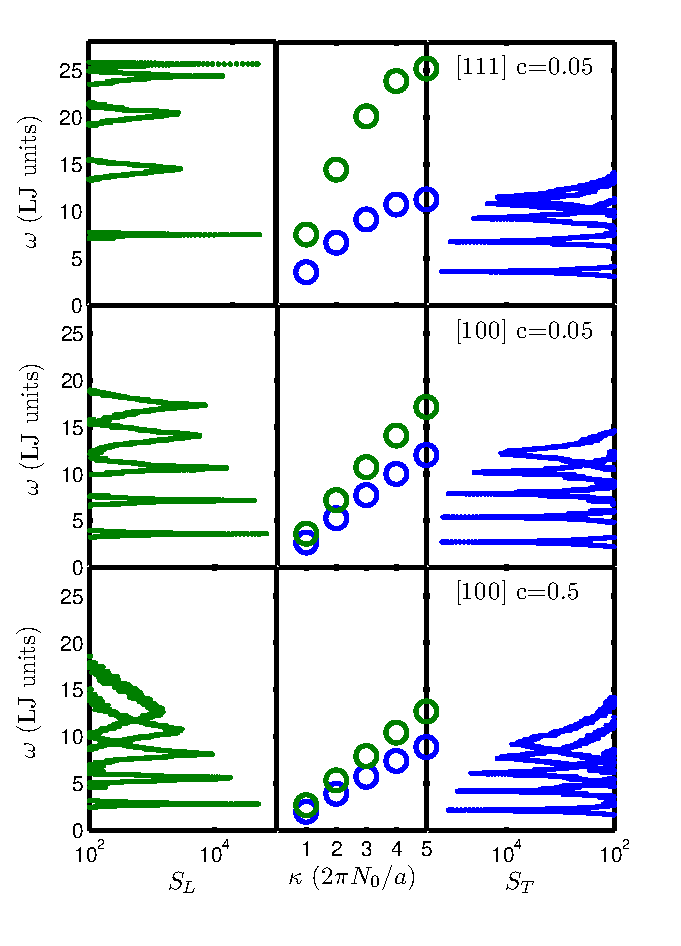
\includegraphics[scale=0.8]
{/home/jason/disorder/lj/alloy/lj_alloy_dsf_100_111.eps}
\vspace*{-5mm}
\end{center}
\caption{\label{F:SF} 
Left and Right Panels: 
The structure factor for logitudinal ($S_L$) 
and transverse ($S_T$) 
polarizations along high symmetry directions ([100], [110] 
where $\mathbf{\kappa}$ = $\pi/a[100]$ and $a$ is the 
lattice constant ) 
of the mass disordered LJ FCC supercells ($c=0.05,0.5$). 
For increasing 
mass disorder $c$, there is a decrease in the center of the peaks 
and an increase in the peak linewdiths. 
Center Panel:
The VC predicted dispersion at the same wavectors used to calculate 
$S_{L,T}$.
}
\end{figure}
%--------------------------------------------------------------------------

%--------------------------------------------------------------------------
\subsection{\label{S:Phonon Lifetimes}Phonon Lifetimes}
%--------------------------------------------------------------------------

%--------------------------------------------------------------------------
\subsubsection{\label{S:From VC Gamma}From VC-NMD and Gamma}
%--------------------------------------------------------------------------

As an alternative to the VC-ALD models for predicting phonon lifetimes 
(Section ), 
we use the normal mode decomposition (NMD) method.(cite) NMD maps the 
atomic trajectories (positions and velocities) of all atoms in an MD 
simulation onto vibrational normal modes.(cite) The MD simulation is 
performed using the perfect (VC) and disordered (Gamma) supercells 
(Section, Fig. ). 
The lifetimes are predicted using the frequencies and eigenvectors 
from both the VC 
($\omega\kv$, $e\kvba$) and the Gamma supercell 
($\omega\kv$, $e\kvba$ with $\mathbf{\kappa}=[000]$). 
The vibrational mode 
frequencies and eigenvectors are necessary 
for the mapping of the atomic trajectories from the MD simulation 
onto the vibrational normal mode coordinates, 
$q\kvt and \dot{q}\kvt$, which are required 
to calculate the total vibrational normal mode energy $E\kv(t)$.(cite)

The normal mode lifetime is predicted using 
\begin{equation}\label{EQ:tau_nmd}
\tau\kv = \int_{0}^{\infty} \frac{<E\kvt E\kvzero>}{ <E\kvzero E\kvzero> }dt.
\end{equation}
For a normal mode which is an exact normal mode of the system, 
the autocorrelation of the total and kinetic  
normal mode energy are cosinusodially damped exponentials 
with a decay time $\tau\kv$ and a single oscillation frequency 
$2\omega\kv$.(cite joe) In Fig. , the 

The effects of disorder enter through the atomic trajectories 
of the MD simulation.

When using the VC normal modes to map the trajectories 
for the explicitly disordered system, 
the mode total and 
kinetic energy do not follow these 
simple functional forms. This can be understood by using spectral NMD 
in the frequency domain, where multiple peaks in an isolated mode's 
energy spectrum ($\Phi$) can be observed (see Fig ).(cite)  
In the case 
of multiple peaks, the choice of which to fit can be ambiguous.  However, 
a lifetime can be predicted unambiguously using Eq. even with 
these multiple-peak artifacts. 
These artifacts are not surprising given two considerations: 
1) the MD simulations 
contain explicit disorder which incluences the atomic trajectories 2)
the normal modes are mapped without using the exact eigenvectors and 
frequencies of the explicitly disordered system. 

The lifetimes predicted using the VC approximation and the Gamma 
supercells are shown in Fig. 
First, the frequencies of the modes for VC-NMD and 
Gamma differ slightly, particularly at high frequency, which is 
demonstrated by the difference in the DOS (Fig. ). 
For a small intervals of frequency, there are a wider range of 
predicted lifetimes for Gamma. This is because there is no symmetry 
averaging of the mode properties, which is performed for the modes 
of the VC.

Descrepencies have been observed previously when the exact normal modes 
of the system are not used.(cite jason) However, the lifetimes predicted 
using VC-NMD are in fairly good agreement with those calculated using 
Gamma (Fig. ). 
Several studies have found good agreement for 
predictions of lifetimes and thermal conductivity 
using non-exact eigenvector mappings
\cite{koker_thermal_2009,thomas_predicting_2010} 
in a wide-range of materials and 
phonon scattering conditions.
\cite{
koker_thermal_2009,thomas_predicting_2010,shiomi_thermal_2011,
ong_reduction_2011,qiu_molecular_2012} 
However, it is crucial 
that results using non-exact mappings are compared to as many 
alternative methods as possible. In this work, VC-NMD is 
compared to the other methods Gamma (Section ), 
GK (Section ), and VC-ALD (Section ).
It is important to remember that the VC normal modes 
are exact in the limit $c->0$. 
Use of the VC 
modes at large $c$ pushes the limits of the approximation, but also 
is useful for predicting an effective group velocity (Section ).

%A general statement from statistical physics
%\cite{rajabpour_thermal_2010} also imposes
%the mode energy autocorrelation to decay exponentially with
%the relaxation time.
%\cite{landau_statistical_1980,srivastava_physics_1990}

%--------------------------------------------------------------------------
\begin{figure}
\begin{center}
\includegraphics[scale=0.75]
{/home/jason/disorder/lj/alloy/m_lj_nmd_xcorr_compare.eps}
\vspace*{-5mm}
\end{center}
\caption{\label{F:NMD XCORR} The spectral energy density $\Phi$ of 
two modes (polarizations $\nu=3,4$ at wavector [0.2 0 0]) calculated 
using VC-NMD for a mass disordered LJ FCC supercell 
($N_0=8$ and $c=0.5$, Section ). 
The VC dispersion-predicted peaks are labeled 
by $\omega_0$. Inset: the same mode's energy 
(kinetic (KE) and total (TE)) autocorrleation functions.  
Note the additional 
harmonic effects in the KE and TE autoccorelation functions 
for $\nu=4$ which are due to the double peaks in $\Phi$. 
A mode lifetime can 
be extracted unambiguously using the integral of the TE autocorrelation 
function (Section ).}
\end{figure}
%--------------------------------------------------------------------------


%--------------------------------------------------------------------------
\begin{figure}
\begin{center}
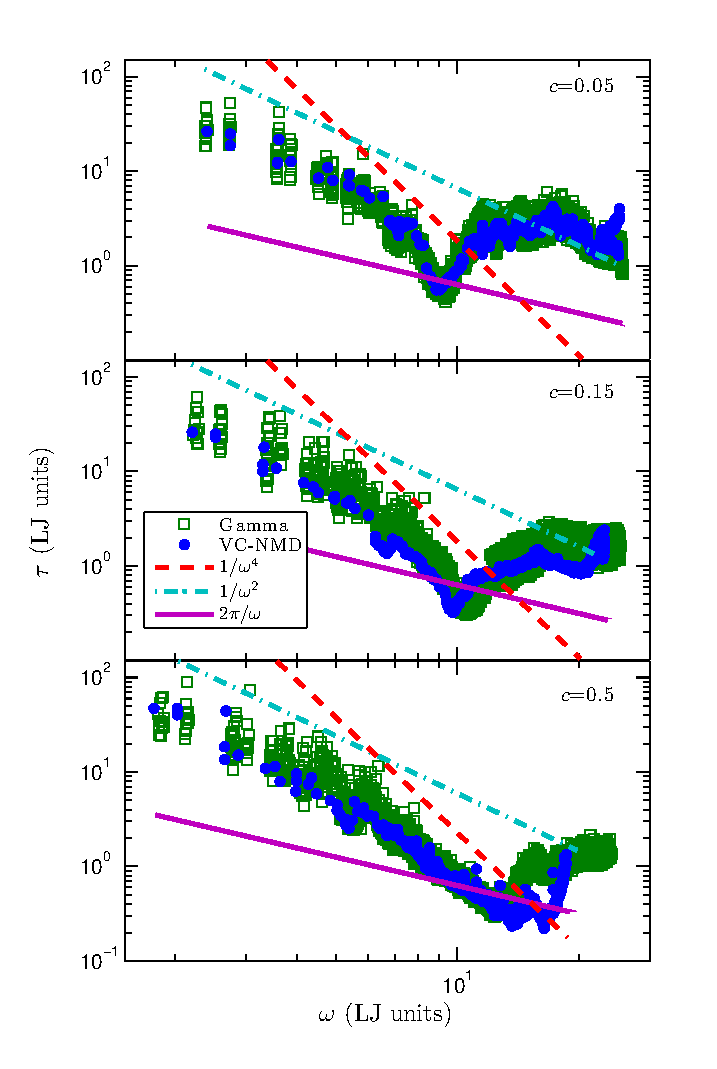
\includegraphics[scale=0.75]
{/home/jason/disorder/lj/alloy/lj_alloy_nmd_vc_gamma_life-2.eps}
\vspace*{-5mm}
\end{center}
\caption{\label{F:VC Gamma life} Lifetimes predicted using VC-NMD 
and Gamma NMD from MD simulations of mass disordered FCC supercells 
(Section ). Both $\omega^{-2}$ and $\omega^{-4}$ scalings can be observed 
at low frequencies, which are predicted by the peturbative models used 
for VC-ALD (Section ). For both VC-NMD and Gamma NMD, most mode 
lifetimes are greater than the Ioffe-Regel limit $\tau = 2\pi/\omega$. 
\cite{taraskin_determination_1999}
While there is more ``noise'' in the Gamma mode data beacuse of the symmetry 
averaging of the VC-NMD modes (Section ), the lifetime magnitudes and 
trends agree well, an important consideration when comparing VC-NMD and 
VC-ALD in Fig. .
}
\end{figure}
%--------------------------------------------------------------------------


%--------------------------------------------------------------------------
\subsubsection{\label{S:From VC-ALD}From VC-ALD}
%--------------------------------------------------------------------------

Assuming the initrinsic and disorder scattering mechanisms 
to operate independently, the 
effective phonon lifetime can be found using Matthiessen's rule(cite),
\begin{equation}\label{EQ:Matthiessen}
\frac{1}{\tau\kv} = \frac{1}{\tau_{p-p}\kv} + \frac{1}{\tau_{d}\kv},
\end{equation}
where $\tau_{p-p}\kv$ accounts for phonon-phonon scattering,
accounts for boundary scattering, $\tau_{d}\kv$ accounts for defect 
scattering.

Phonon-phonon scattering ($\tau_{p-p}\kv$) is typically treated 
using anharmonic perturbation theory (ALD) including only 3-phonon 
processes.\cite{turney_predicting_2009,garg_role_2011,tian_phonon_2012} 
It has been estimated that the effects of higher order phonon 
processes are small \cite{ecsedy_thermal_1977}, particularly at 
low temperatures.\cite{turney_predicting_2009} At low frequencies,
$\tau_{p-p}\kv$ follows a scaling due to both normal ($B_1\omega^2$) 
and umklapp ($B_2\omega^2$) 3-phonon scattering processes, where 
the density of states is Debye-like(cite) and the 
constants $B_1$ and $B_2$ are typically fit to experimental data.
The scaling $\tau ~ \omega^{-2}$ can be observed  
in both the NMD (Fig. ) and ALD (Fig. ) predicted results. 

Using harmonic perturbation theory, Tamura gives a general expression 
for mass point defect scattering\cite{tamura_isotope_1983}
\begin{equation}\label{EQ:tau_d}
\begin{split}
\frac{1}{\tau_{d}\kv} = \frac{\pi}{2N}\omega^2\kv 
\sum_{\mathbf{\kappa'}\nu'} \delta( \omega\kv - 
\omega\kvp ) \\
\sum_{b} g(b) 
|e^*\kvbap \cdot e\kvba |^2 ,
\end{split}
\end{equation}
where 
$g(b) = \sum_\mu c^{\mu}(b)(1-m^{\mu}(b)/\bar{m}(b))^2$, 
N is the number of unit cells, and $c^\mu$ is the concentration, 
$m^\mu(b)$ is the mass of the $\mu$-th species 
and $\bar{m}^{\mu}$ is the average mass. 
For the binary alloys considered, 
there is one atom type in the unit cell ($b=1$ only) 
with $\mu=a,b$, such that the alloying atom labeled by $m^b_{1-c}$ 
can be considered to be an ``isotope'' of atom labeled 
$m^a_{c}$.  This convention is appropriate because of the 
perturbative approach used to derive Eq. , while we consider 
large disorder of up to $c=0.5$.\cite{tamura_isotope_1983}

By considering the symmetry properties of the FCC lattices 
considered in this work (Section ), it can be shown that  
$1/\tau_{d}\kv =\frac{\pi}{2} g \omega^2\kv D(\omega\kv)$, where 
$D(\omega\kv)$ is the density of states (Section ) 
and $g$ is the disorder coupling strength.\cite{tamura_isotope_1983}   
Under the Debye-approximation ($D(\omega\kv)~\omega^{2}$), 
the phonon scattering due to mass point-defects 
is given by $A\omega^{-4}$, where $A$ is a constant related to the unit 
cell volume, branch-averaged group velocity, and disorder coupling strength 
($g$ in Eq. above). 
The frequency dependence ($\omega^4$) is the same as 
Rayleigh scattering, which is valid at low frequency and observed 
in both the NMD (Fig. ) and ALD (Fig. ) predicted results. 













The disorder 
scattering scaling is expected to fall off faster than $\omega^{-4}$ 
when $D(\omega\kv)$ grows faster than the Debye scaling of 
$\omega^{2}$ (Fig. , Section ). 
The lifetimes do fall off faster $\omega^{-4}$ for the 
mass disordered LJ FCC supercells for a narrow range of 
frequencies near $\omega = 10$ in Fig. for $c=0.05,0.15$, 
but seem to follow more closely $\omega^{-4}$ for $c=0.5$. 

Bond disorder 
can be accounted for using a similar expression with an average
atomic radius or suitable scattering cross-section.
\cite{klemens_scattering_1955,klemens_thermal_1957} 
The effect of bond and mass disorder has been investigated computationally 
by Skye and 
Schelling for Si/Ge \cite{skye_thermal_2008}, 
where it was shown that mass disorder is 
the dominant scattering mechanism. In this work we consider only 
mass disorder.

For the VC-ALD method, 
the intrinsic $\tau\kv_{p-p}$ is calculated using the method described in.
\cite{turney_predicting_2009}
To calculate the disordered lifetimes $\tau\kv_{d}$ (Eq. ), 
it is necessary to broaden 
the $\delta$ function using a Lorentzian function. 
For all calculations, the Lorentzian was broadened using a value of $100$ 
times the mean level spacing. For the system sizes here, 
the results do not differ significantly 
if this broadening value is varied by changing it manually or making 
the system size ($N_0$) bigger.

%--------------------------------------------------------------------------
\subsection{\label{S:Vibrational Mode Diffusivity}
Vibrational Mode Diffusivity}
%--------------------------------------------------------------------------

The diffusivity section was a bit hard to follow.

In the classical limit, where the specific heat $c_p\kv = k_{B}$, 
a vibrational mode's contribution to thermal 
conductivity is determined by the mode thermal diffusivity. For 
phonons, the thermal diffusivity is 
\begin{equation}\label{EQ:Dph}
D_{ph}(\omega\kv) = \pmb{v}^{2}_{g,\mathbf{n}}\kv \tau\kv.
\end{equation}


We now compare the phonon mode diffusitivies, $D_{ph}(\omega\kv)$
predicted by both VC-NMD and VC-ALD to the proposed lower limit 
$D_{AF,HS} = (1/3)v_sa$ (see Section ).  
Here, $a$ is $1/2$ the lattice constant of the 
cubic conventional unit cells used for both FCC LJ argon and diamond-FCC 
SW silicon, although the choice of this length scale is not unique.
For the a value in Eqs. (12)-(14), why not use the bond length?

For LJ argon, VC-NMD predicts lifetimes which 
are generally larger than the period 
($2\pi/\omega\kv$)
of the vibrational oscillation (Ioffe-Regel limit)(cite), 
and actually increase high frequency for small intervals (Fig. and ). 
VC-NMD predicts larger phonon lifetimes at high 
frequency compared to VC-ALD (Fig. ), which predicts 
essentially monotonically 
decreasing lifetimes with increasing frequency. Because VC-NMD and VC-ALD 
use the same values for $v_g\kv$, the phonon mode 
diffusivities $D_{ph}$ are also underpredicted by VC-ALD compared to VC-NMD. 
This leads to an 
underprediction for VC-ALD 
of both the thermal conductivity spectrum (Fig. ) at high 
frequency and the total thermal conductivity (Fig. ) compaed to VC-NMD. 

For both VC-NMD and VC-ALD, a significant number of modes have 
$D_{ph} \lt D_{AF,HS}$. This leads to an underprediction of the 
total thermal conducitvity compared to GK (Fig. ). The diffusivity of these 
modes can be adjusted such that any mode with $D_{ph} \lt D_{AF,HS}$ is 
given $D_{ph} = D_{AF,HS}$.  The result of this adjustment, referred to as 
VC-NMD* and VC-ALD*, is examined 
in the next section.

%--------------------------------------------------------------------------
\begin{figure}
\begin{center}
\includegraphics[scale=0.75]
{/home/jason/disorder/lj/alloy/af_nmd_ald_tau_diff_kw_c05_3-2.eps}
\vspace*{-5mm}
\end{center}
\caption{\label{F:Dph_lj} gamma point results}
\end{figure}
%--------------------------------------------------------------------------

%--------------------------------------------------------------------------
\begin{figure}
\begin{center}
\includegraphics[scale=0.75]
{/home/jason/disorder/si/alloy/af_nmd_ald_tau_diff_kw_c05_2-2.eps}
\vspace*{-5mm}
\end{center}
\caption{\label{F:Dph_si} gamma point results}
\end{figure}
%--------------------------------------------------------------------------

The energy diffusivity, d͑␻͒, quantifies how far a wave
packet narrowly peaked at a frequency ␻ can propagate.
\cite{allen_thermal_1993,xu_energy_2009,vitelli_heat_2010}

A heuristic ar-
gument for the relation between d͑␻͒ and ␬͑T͒ is as follows.
For a system in a temperature gradient, it is well known that
the heat diffusivity obeys the relation d = ␬V / C. Thus,
␬ = dC / V. This relation can be generalized mode by mode.

In amorphous systems, the diffusivities themselves can be combined 
using a Matthiesen-like expression (multiple resistors in series).
\cite{tritt_thermal_2005}

The mode lifetime typically diverges as $\omega -> 0$ because
the vibrational modes are long-wavelength plane waves (phonons) 
that weakly scattered by the disorder.\cite{sheng_introduction_2006} 



In fact, the low-temperature behavior of glasses is described 
\cite{graebner_phonon_1986}

At very low frequency, the mode diffusivities for phonons or diffusons 
can be factored as the product of the sound speed, 
$D_{ph} = v_s^2\kv\tau\kv$ and $D_{AF} = (1/3)(v_s)^2\tau_{AF}$.


The key difference is that for the lattices studied in this work, 
for $c=0$ there is dispersion such that $v_g\kv$ instead of 
$v_g\kv = v_s$ as in the Cahill-Pohl model. For perturbative 
disorder ($c=0.05$ Fig. ), the narrow peaks of the disordered 
lattice's structrue factor (Section ) suggest that the

This perplexing property of glasses
has been explained heuristically by assuming that phonons
are scattered so strongly by structural disorder that trans-
port becomes diffusive, with a frequency regime of small,
constant thermal diffusivity 
\cite{kittel_interpretation_1949,zhou_heat_1991}

By contrast,
␬͑T͒ is generally infinite if anharmonic corrections are ig-
nored. This is because d͑␻͒ in the integrand of Eq. ͑4͒ di-
verges too strongly at low ␻ due to phonons that are progres-
sively less scattered with increasing wavelength.
\cite{vitelli_heat_2010} 
In order to cure this divergence, additional scattering
mechanisms, beyond harmonic theory, are typically invoked
resulting in an additional contribution to the diffusivity,
dc͑␻͒




In heavily disordered systems, such as large $c$ alloys or glasses, 
modes can transport heat by harmonic coupling due to the disorder 
in the Allen-Feldman (AF) theory of diffusons.\cite{allen_thermal_1993}  
In the classical limit, 
the AF thermal 
conductivity is written as
\begin{equation}\label{EQ:M:k_HS}
k_{AF} = \sum_\omega  \frac{k_{B}}{V} D_{AF}(\omega\kv),
\end{equation}
where $V$ is the system volume and $D_{AF}(\omega_{AF})$ is the thermal 
diffusivity of the mode labeled by frequency 
$\omega\kv$ with 
$\nu$ ranging over all 
modes in the disordered supercell and $\mathbf{\kappa} = [000]$.(cite) 

In a weakly scattering system, $D_{AF} = v_s \tau(\omega)/3$
\cite{xu_energy_2009}

In fact, for a-Si, the mode diffusivities do vary as a function 
of frequency, which is used to explain the propagating 
mode effects seen in a-Si thin films.(cite)

In the high-scatter (HS) limit,(cite) the AF diffusivity of each mode is
\begin{equation}\label{EQ:M:k_HS}
D_{AF,HS} = \frac{1}{3} v_s a.
\end{equation}
A similar HS limit for mode diffusivity 
is given by the Cahill-Pohl (CP) model,(cite)  
\begin{equation}\label{EQ:M:k_HS}
D_{CP,HS} = 0.403 v_s a.
\end{equation}
The CP thermal conductivity prediction in the HS limit is
\begin{equation}\label{EQ:M:k_HS}
k_{CP,HS} = (\frac{\pi}{6})^{1/3} (\frac{3}{2}) \frac{k_{B}}{V_b}b v_s a,
\end{equation}
where $V_b$ is the volume of the unit cell, $v_s$ is the 
branch-averaged sound speed, and $a$ is the lattice constant 
(or appropriate length scale).\cite{cahill_lattice_1988} 
Comparing with Eq., the AF,HS limit predicts a mode diffusivity and 
thermal conductivity which is approximately $\%20$ smaller then 
CP,HS.\cite{cahill_lattice_1988} 
Ignoring this small difference, 
the interpretation for both $D_{AF,HS}$ and $D_{CP,HS}$ is of a vibrational 
mode with a group velocity equal to the sound speed 
and mean-free path equal to the 
lattice spacing. 
While the CP,HS model assumes $\tau\kv = 1/\omega\kv$ 
and $v_g = v_s$ for all modes, the AF theory is capable 
of predicting the mode diffusivities without 
any assumptions other than a harmonic approximation.(cite)

With sufficient disorder, the 
harmonic AF theory is capable of accurately predicting a finite 
thermal conductivity.
\cite{feldman_thermal_1993,shenogin_predicting_2009} 
However, the AF theory does not 
treat the intrinisic anharmonic scattering of low frequency 
phonon modes, where in the infinite-size   
the AF conductivity of a disordered lattice is divergent.(cite)   
While the low frequency modes are not treated properly in the harmonic 
AF theory, the mode diffusivities 
$D_{AF}$ of high frequency modes in the heavily disordered ($c=0.5$) LJ 
FCC supercell approach that of similar frequency modes in the 
amorphous phase 
(Fig. ).
%\footnote{
footnote(The amorphous LJ phase was created by liquifying the crystal 
and instantly quenching by removing all kinetic energy.  The resulting 
structure was then energy minimized and annealed in an NPT ensemble at 
zero pressure and $T=10$ K.(cite lammps)
%}
In the amorphous phase, modes with significant 
contribution to thermal transport can be modeled using a mode-independent 
diffusivity of $D_{AF,HS}$ (Eq. ). In fact, the difference between  
$k_{AF} = 0.099 W/m=K$ and $k_{HS,CP} = 0.124$ is approximately 
$\%20$. 
This places a plausible lower-bound on the value of the phonon mode 
diffusivities, $D_{ph} \ge D_{AF,HS}$, predicted by VC-NMD and VC-ALD in 
the following section.

%--------------------------------------------------------------------------
\begin{figure}
\begin{center}
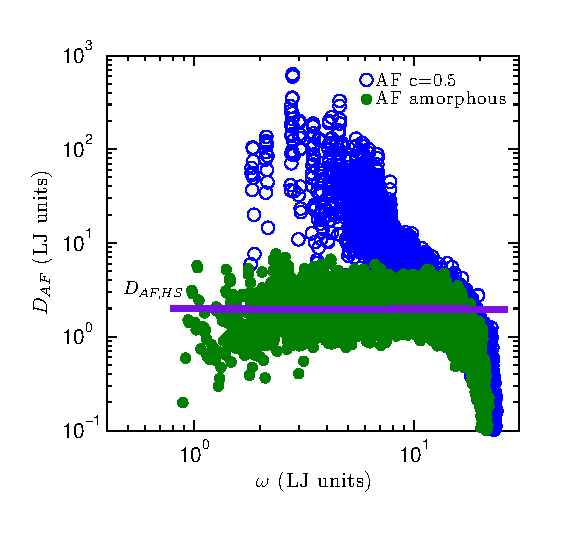
\includegraphics[scale=0.75]
{/home/jason/disorder/lj/alloy/af_c5_amor_DAF_kw_2.eps}
\vspace*{-5mm}
\end{center}
\caption{\label{F:AF} gamma point results}
\end{figure}
%--------------------------------------------------------------------------


%--------------------------------------------------------------------------
\section{\label{S:Thermal Conductivity}Thermal Conductivity Predictions}
%--------------------------------------------------------------------------
An addition of as little as 10\% Ge is sufficient to reduce the thermal 
conductivity to the minimum value achievable through alloying. 
Theoretically, mass disorder is found to increase the 
anharmonic scattering of phonons 
through a modification of their vibration eigenmodes. 
Notably, the thermal conductivity is found
to drop sharply after only a small amount of alloying. This
is due to the strong harmonic scattering of phonons even
in the dilute alloy limit.

Duda shows that taking a perfect alloy and disordering via an order 
parameter allows control of thermal conductivity.
\cite{duda_controlling_2012}

In fact, the beginning breakdown of the intrinsic scattering model 
($\tau_{p-p}\kw$) can be observed for the perfect ($c=0.0$) crystal at 
$T=40$ K (see Fig. ), where ALD begins to overpredict compared to GK.  This 
can be explained by the emerging importance of higher order (n$> 3$) 
n-phonon process at high temperatures.\cite{turney_predicting_2009}

For LJ argon, bulk thermal conductivity predictions are made for 
VC-NMD, VC-ALD and GK (Fig. ). For SW silicon, bulk thermal conductivity 
predictions can only be made for VC-ALD and GK (see Appendix ). 
For LJ argon, both VC-NMD and VC-ALD underpredict the thermal 
conductivity compared to GK. By adjusting the mode diffusivity 
$VC-NMD*$ and $VC-ALD*$.



%--------------------------------------------------------------------------
\begin{figure}
\begin{center}
\includegraphics[scale=0.75]
{/home/jason/disorder/lj/alloy/lj_cond_compare.eps}
\vspace*{-5mm}
\end{center}
\caption{\label{F:conductivity_lj} The vibrational conductivity of LJ alloys 
predicted using MD simulations and the Green-Kubo method. The predicted 
thermal conductivities are for a LJ alloy of the form $m^a_{1-c}m^b_{c}$, 
where $m^a =$ 1, $m^b=$ 3, and $m_r = m^a/m^b=$ 3 (in LJ units). As the 
alloy concentration is increased perturbatively, the vibrational 
conductivity drops quickly and saturates to a minimum at $c=0.5$. For 
$c=0.5$ the system is heavily disordered and the vibrational conductivity 
approaches that of an amorphous system.}
\end{figure}
%--------------------------------------------------------------------------

%--------------------------------------------------------------------------
\begin{figure}
\begin{center}
\includegraphics[scale=0.75]
{/home/jason/disorder/si/alloy/si_cond_compare.eps}
\vspace*{-5mm}
\end{center}
\caption{\label{F:conductivity_si} The vibrational conductivity of LJ alloys 
predicted using MD simulations and the Green-Kubo method. The predicted 
thermal conductivities are for a LJ alloy of the form $m^a_{1-c}m^b_{c}$, 
where $m^a =$ 1, $m^b=$ 3, and $m_r = m^a/m^b=$ 3 (in LJ units). As the 
alloy concentration is increased perturbatively, the vibrational 
conductivity drops quickly and saturates to a minimum at $c=0.5$. For 
$c=0.5$ the system is heavily disordered and the vibrational conductivity 
approaches that of an amorphous system.}
\end{figure}
%--------------------------------------------------------------------------


%--------------------------------------------------------------------------
\section{\label{S:Discussion}Discussion}
%--------------------------------------------------------------------------



While the models presented in, there is no theoretical justification for 
the lower limit to the the mode mean-free path.\cite{graebner_phonon_1986} 
For the lattices studied in this work, the more appropriate quantity to 
consider is the mode diffusivity since both the 
effective mode lifetime   
and group velocity are varying with frequency (Fig. ). 
Since the Allen-Feldman theory does not rely on the assump-
tion of propagating phonons we expect the results for d͑␻͒
to be valid even in the high-frequency regime, where the
diffusivity cannot be factorized into a product of $l(\omega)$ times
a frequency-independent speed of sound.


For $c=0$ the group velocities are given from the dispersion (Section ). 

In these ordered and disordered lattices, it is difficult to separate 
the contributions to the total vibrational 
conductivity from $D_{ph}\kv$ and $D_{AF}$ unless the lower limit 
$D_{CP,HS}$ or $D_{AF,HS}$ are used.  

While the
expression for harmonic defect scattering (Eq.) is valid for
perturbative disorder, its use leads to good agreement with
several experimental and computational results with large disorder.  
Cahill shows that conductivty reduction in dilute 
Ge-doped Si epitaxial layers 
is captured by mass perturbative disorder.\cite{cahill_thermal_2005} 
In this case, the mass disorder is large ($m_{Ge}/m_{Si} = 2.6$) 
but the overall disorder strength is dictated by the concentration. 
For example, as little as $6.2\times10^{19} cm^{-3}$ Ge
($g = 3.1\times10^{-3}$) is enough to reduce the thermal conductivity of 
Si by almost a factor of 2.\cite{cahill_thermal_2004}
In the
case of the $Ni_{0.55}Pd_{0.45}$ alloy, the atomic species
are chemically similar but both the mass disorder 
($m_{Pd}/m_{Ni} \approx 2$) and concentration are large ($g=0.078$) 
and good agreement is seen with the Eq. .
\cite{kamitakahara_vibrations_1974}

While , the effect of explicit disorder has been demonstrated in the 
calculation of the intrinsic phonon lifetimes.\cite{garg_role_2011}

Experimental measurements of isotopically pure and Ge-doped 
Si epitaxial layers demonstrate the original theory by Abeles can predict 
thermal conductivity in dilute alloys. Abeles also found good agreement 
with dilute predictions for both experimental measurements of both 
Si-Ge alloys and also (Ga,In)As alloys.\cite{abeles_lattice_1963} However, 
both of these alloy systems have a relatively high thermal conductivities 
(on the order of 1-10 W/m-K at 300 K). However, in the heavily disordered 
system In(As,P) (mass ratio of 3.7) worse agreement with the Abeles theory 
is observed. 

The theory by Tamura is able to treat disorder scattering in an arbitrary 
crystal with dispersion. The theory, however, fails to predict the 
lifetimes of high-frequency modes, which are critical to the total 
thermal conductivity in LJ argon (see Fig. and ). To match the predicted 
phonon lifetime at high fequency for $c=0.05$ 
($\tau\kv \propto const.$, Fig. ), 
the Tamura theory requires a DOS which scales as 
$D(\omega\kv) \propto const.$. Clearly from Fig. , this is not the case 
with either the VC or Gamma modes. To match the predicted 
phonon lifetime at high fequency for $c=0.5$ 
($\tau\kv \propto 1/\omega\kv$, Fig. , also true for all $c$ in SW silicon), 

While Broido found that omission of optical scattering overpredicts 
the thermal 
conductivity of bulk Si by a factor of 2-3, 
optical modes contribute less than $5\%$ 
to thermal conductivity itself. Similarly, the diffusivity adjusted thermal 
cobductivities of SW Si are increased by less then $5\%$, demonstrating the 
unimportance of the high frequency ``optical'' modes in SW Si alloys.

the problem is with taud.  VC-NMD agrees well with GK for both LJ and SW, 
while ALD-taud underpredcits for LJ.  VC-NMD and ALD-taud use the same 
group velocity and classical specific heat.

Particularly challenging is predicting a representative group velocity 
for modes in a disordered systems. 
Use of the VC approximation is a theoretically and 
computationally simple way to predict a representative group velocity.

High thermal conductivity materials tend to have a conductivity spectrum 
which is peaked in the low frequency range.(cite) 
It is in this range where the mode 
lifetimes follow closely the scalings with frequency which can be 
predicted by treating intrinsic and disorder scattering as 
perturbations (Eq. ).

In contrast, 
in LJ argon the high frequency phonon mode properties are critical 
to the thermal transport.(cite)  
While the low frequency phonon properties predicted by VC-NMD and 
VC-ALD agree, it is the failure of the perturbative models at 
high frequency which causes VC-ALD to underpredict. The failure 
to account for harmonic disordered scattering due to the AF theory 
is responsible for causing both VC-NMD and VC-ALD to underpredict 
versus GK, which affects the high frequency modes significantly. 
LJ argon, with lower 
frequencies, lifetimes, and group velocities compared to 
``stiff'' SW silicon, 
is considered a ``soft'' system. The predictions using 
VC-NMD, VC-ALD demonstrate the importance of explicit disorder 
modeling in ``soft'' systems and possible underprediction 
of the thermal properties.\cite{tian_phonon_2012}

For SW silicon, the low frequency modes dominate thermal transport 
even in the heavily disordered alloy.(cite new Hopkins) 
It is thus unsurprising that predictions for 
SW silicon using VC-ALD agree well with VC-NMD and GK. This is also a 
plausible explanation for the success of predictions using 
VC-ALD and ab initio calculations compared to experiment for 
``stiff'' systems (i.e. Si-Ge, GaN, and Diamond).(cite)

In SW silicon even the amorphous phase has significant contributions 
from propagating modes which can be considered to be phonons. This is 
can seen by comparing the thermal conductivity predicted for the 
SW silicon amorphous phase ($k_{GK} =$ 3 W/m-K (cite)) compared to 
$k_{CP,HS} = $0.5 W/m-K.  For LJ argon in the amorphous phase, 
$k_{GK} = $0.121 W/m-K and $k_{CP,HS} =$ 0.12 W/m-K, indicating that 
all important modes to thermal transport are non-propagating.

%--------------------------------------------------------------------------
\section{\label{S:}Summary}
%--------------------------------------------------------------------------



%--------------------------------------------------------------------------
\appendix
%--------------------------------------------------------------------------

%--------------------------------------------------------------------------
\section{\label{A:Finite Simulation-Size}
Finite Simulation-Size Scaling for Thermal 
Conductivity}
%--------------------------------------------------------------------------
To predict a bulk thermal conductivity, extrapolation is used by the 
following finite size scaling $ 1 / k \propto 1/N_0$. For VC-NMD and 
VC-ALD, the validity of this finite-size scaling 
is the low frequency modes in the finite system must be dominated by 
intrinsic scattering such that $\tau\kv \propto \omega\kv^{-2}$ 
and approximately follow the Debye approximation 
with respect to $v_{g,\mathbf{n}}$ and DOS $D(\omega\kv)$.
\cite{shiomi_thermal_2011} For LJ 
argon, this requirement is satisfied for modest system sizes 
(for $N_0 = 6$ to $12$) so that both VC-NMD and VC-ALD predictions 
can be extrapolated to a bulk value. 
For SW silicon, the thermal conductivity is dominated by low-frequency 
modes (Fig. ). Becasue of this, large system sizes 
(up to $N_0 = 24$) are needed to satsify the 
extrpaolation requirements and only VC-ALD can be used.(cite) This 
underlines the computational efficieny of the VC-ALD method which is 
necessary when computationally expensive 
ab initio methods are used (Section ).
\cite{garg_role_2011,tian_phonon_2012,
lindsay_thermal_2012,esfarjani_heat_2011} 
For the GK method, the finite size extrapolation is used for 
both LJ argon and SW silicon for smaller system sizes $N_0 \le 12$. 
The validity of this result can be explained in terms of a 
combination of effects which are specific to the MD simulations.
\cite{esfarjani_heat_2011} In fact, for $c=0$ the GK results are independent 
of system size for $N_0 = 4$ to $N_0 = 12$ for both LJ argon and SW silicon.

\clearpage
\bibliographystyle{apsrev}
%\bibliography{/home/jason/sed/jop/asme_prb_paper/prb/references}
\bibliography{/home/jason/Dropbox/book/ntpl-120512}
\end{document}
